
\subsection{Microbenchmark performance}
\label{subsec:microbench}

The two dominant factors that determine \JV update time are the time to
perform a GC, determined by the number of objects, and the time to run
object transformers, determined by the fraction of objects being updated.
To measure each cost, we devised a simple microbenchmark that
creates an array of objects and transforms a specified fraction of these
objects when a dynamic software update is triggered. The microbenchmark has
two simple classes, \texttt{Change} and \texttt{NoChange}. Both contain
three integer fields, and three reference fields that are always {\tt
null}. The update adds an integer field to {\tt Change}. The user-provided
object transformation function copies the existing fields and initializes
the new field to zero.
% The benchmark contains two arrays, one for \texttt{Change} objects and
% one for \texttt{NoChange} objects.
We measure the cost of performing an update while varying the total number
of objects and the fraction of objects of each type. The number of objects
is the maximum that can fit in heap sizes 32, 64, 128 and 256 MB\@.  Note
that \RVM's heap includes \VM data structures as well. We measure the
running time in a generous heap, five times the minimum required size, such
that the only collections are those DSU triggers. We report the median of
21 runs.

% \begin{sidewaystable}
% \centering
% \begin{footnotesize}
% \begin{tabular}{|r|r|rrrrrrrrrrr|}
%                                                                                                                                    \hline
% \multirow{2}{*}{\# objects}     & \mc{1}{c}{Heap}   & \mc{11}{|c|}{Fraction of updated objects \T}                              \\
%                                 & \mc{1}{c|}{size}  &
%                        0\%  &   10\%  &   20\%  &   30\%  &   40\%  &   50\%  &   60\%  &   70\%  &   80\%  &   90\%  &  100\%  \\ \hline
% \mc{13}{|c|}{Garbage collection time (ms) \T}                                                                                   \\ \hline \T
%  280000 &  160 MB &    78.2 &    81.3 &    83.1 &    89.3 &    99.0 &   103.2 &   108.3 &   113.2 &   113.3 &   120.3 &   120.0 \\
%  770000 &  320 MB &   148.9 &   165.0 &   181.9 &   195.8 &   213.2 &   223.2 &   237.0 &   249.0 &   262.0 &   269.5 &   278.6 \\
% 1760000 &  640 MB &   313.3 &   347.7 &   382.9 &   416.0 &   449.8 &   478.9 &   506.8 &   534.0 &   558.8 &   583.7 &   601.5 \\
% 3670000 & 1280 MB &   615.4 &   694.6 &   763.0 &   833.6 &   900.1 &   965.9 &  1019.0 &  1076.4 &  1129.9 &  1181.2 &  1217.5 \\ \hline
% \mc{13}{|c|}{Running transformation functions (ms) \T}                                                                          \\ \hline \T
%  280000 &  160 MB &     0.1 &    13.0 &    23.2 &    34.6 &    43.9 &    54.0 &    62.7 &    74.5 &    84.1 &    93.9 &   104.2 \\
%  770000 &  320 MB &     0.1 &    33.7 &    63.1 &    91.2 &   116.8 &   145.4 &   173.9 &   201.0 &   231.3 &   262.0 &   292.6 \\
% 1760000 &  640 MB &     0.1 &    77.9 &   143.9 &   207.7 &   269.5 &   333.7 &   397.6 &   464.0 &   534.6 &   604.5 &   674.9 \\
% 3670000 & 1280 MB &     0.1 &   160.8 &   299.2 &   429.4 &   560.2 &   693.8 &   827.3 &   975.0 &  1119.6 &  1263.7 &  1405.4 \\ \hline
% \mc{13}{|c|}{Total DSU pause time (ms) \T}                                                                                      \\ \hline \T
%  280000 &  160 MB &    82.8 &    99.0 &   109.5 &   128.0 &   147.6 &   161.2 &   174.5 &   192.8 &   202.5 &   218.8 &   228.1 \\
%  770000 &  320 MB &   153.6 &   202.9 &   249.0 &   291.4 &   334.5 &   372.6 &   414.8 &   455.4 &   498.1 &   535.3 &   576.8 \\
% 1760000 &  640 MB &   316.6 &   429.5 &   530.5 &   627.2 &   723.4 &   816.0 &   908.6 &  1002.6 &  1097.5 &  1191.5 &  1281.2 \\
% 3670000 & 1280 MB &   618.7 &   859.0 &  1065.9 &  1269.9 &  1466.1 &  1663.6 &  1850.8 &  2054.2 &  2253.1 &  2448.5 &  2627.9 \\ \hline
% \end{tabular}
% \end{footnotesize}
% \caption{Microbenchmark results: \JV update pause time (in ms) for various heap sizes}
% \label{tab:microbench}
% \end{sidewaystable}

\begin{sidewaystable}
\newcommand{\GcTime}{\multirow{4}{0.15\textwidth}{Garbage collection time (ms)}}
\newcommand{\TfTime}{\multirow{4}{0.15\textwidth}{Running transformation functions (ms)}}
\newcommand{\ToTime}{\multirow{4}{0.15\textwidth}{Total DSU pause time (ms)}}
\centering \footnotesize
\begin{tabular}{*{14}{r}} \toprule
\mc{1}{c}{\# objects}     & \mc{1}{c}{Heap}  && \mc{11}{c}{Fraction of updated objects}                              \\
\mc{1}{c}{in '000s}       & \mc{1}{c}{(MB)}  &&
              \T 0\%  &   10\%  &   20\%  &   30\%  &   40\%  &   50\%  &   60\%  &   70\%  &   80\%  &   90\%  &  100\%  \\ \midrule
  280 &   160 & \GcTime &    78 &    81 &     83 &    89 &    99 &   103 &   108 &   113 &   113 &   120 &   120 \\
  770 &   320 &         &   148 &   165 &    181 &   195 &   213 &   223 &   237 &   249 &   262 &   269 &   278 \\
1,760 &   640 &         &   313 &   347 &    382 &   416 &   449 &   478 &   506 &   534 &   558 &   583 &   601 \\
3,670 & 1,280 &         &   615 &   694 &    763 &   833 &   900 &   965 &  1019 &  1076 &  1129 &  1181 &  1217 \\ \midrule
  280 &   160 & \TfTime &     0 &    13 &     23 &    34 &    43 &    54 &    62 &    74 &    84 &    93 &   104 \\
  770 &   320 &         &     0 &    33 &     63 &    91 &   116 &   145 &   173 &   201 &   231 &   262 &   292 \\
1,760 &   640 &         &     0 &    77 &    143 &   207 &   269 &   333 &   397 &   464 &   534 &   604 &   674 \\
3,670 & 1,280 &         &     0 &   160 &    299 &   429 &   560 &   693 &   827 &   975 &  1119 &  1263 &  1405 \\ \midrule
  280 &   160 & \ToTime &    82 &    99 &    109 &   128 &   147 &   161 &   174 &   192 &   202 &   218 &   228 \\
  770 &   320 &         &   153 &   202 &    249 &   291 &   334 &   372 &   414 &   455 &   498 &   535 &   576 \\
1,760 &   640 &         &   316 &   429 &    530 &   627 &   723 &   816 &   908 &  1002 &  1097 &  1191 &  1281 \\
3,670 & 1,280 &         &   618 &   859 &   1065 &  1269 &  1466 &  1663 &  1850 &  2054 &  2253 &  2448 &  2627 \\ \bottomrule
\end{tabular}
\caption{Microbenchmark results: \JV update pause time (in ms) for various heap sizes}
\label{tab:microbench}
\end{sidewaystable}

% vim:tw=0

\begin{figure}[t]
\begin{center}
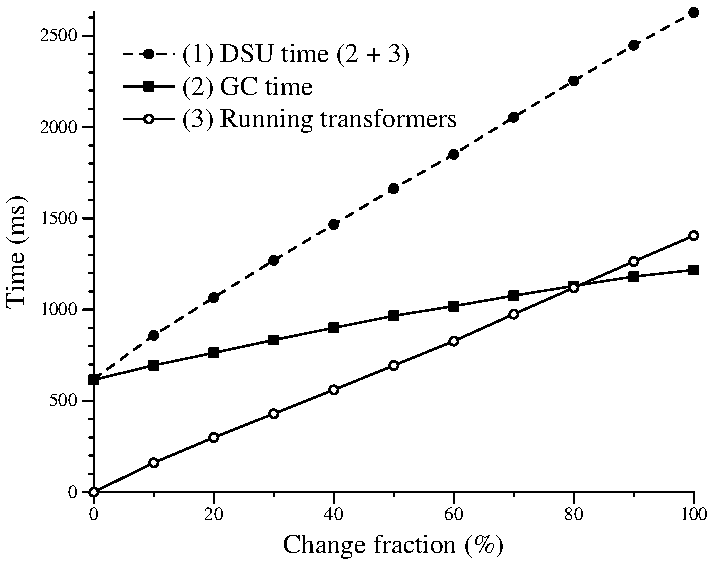
\includegraphics[scale=0.73]{100-graphs/microbench}
\hangcaption{Microbenchmark pause times with a heap size of 1280 MB containing
3.67 million objects\label{fig:microbench}}
\VspaceFixForHangcaption
\end{center}
\end{figure}


Table~\ref{tab:microbench} shows the elapsed time while varying the number
of total objects and the fraction of the objects that are updated.  The
variance was insignificant, so we do not report it.  The first group of
rows reports garbage collection time, the second group reports the time to
transform all updated objects, and the final group reports the total update
time. While the total time includes the time to load and install the
updated classes, synchronize running threads, and find a DSU safe point, it
is roughly equal to the sum of GC time and transformation time.  The first
column of the table shows the number of objects in the test, and the second
column the heap size, which is five times the minimum heap size to run the
microbenchmark. Columns 4 though 14 show pause times for varying fractions
(from 0\% to 100\%) of updated objects. 

To shed light on the results in the table, Figure~\ref{fig:microbench}
plots collection time, transformer time, and total update time for the
microbenchmark with 3.67 million objects in a 1280 MB heap.  The figure
shows that the costs of garbage collection and transformation increase  as
a function of the number of changed objects.  The slope of the ``GC time''
line illustrates the cost to deal with one object of the update type.  This
cost includes creating an additional copy of the transformed object;
creating an update log entry with a pointer to the old and new copy; and
caching a pointer to the old copy from the new copy. The slope of the
``Running transformers'' line illustrates the cost of accessing the update
log and actually running the transformer for one object.  This extra
processing to handle transforming objects increases the total pause time
with all objects updated by roughly four times compared to the pause time
with no object updated.  The ``Running Transformers'' line is steeper than
the ``GC time'' line, revealing that the cost of running transformers is
higher than the extra copying cost incurred during GC\@.

Transformations are more expensive than standard copying GC. The GC uses a
highly optimized {\tt memcopy} like code, whereas our transformer functions
use reflection to look up the \texttt{jvolveObject} function of the right
type, and this function copies one field at a time. One optimization would
be to eliminate the log by copying the old and new objects to their own
space and walking through and transforming each object.  The cost of
reflection could be reduced by caching the lookup, but even then a
na\"ively compiled field-by-field copy is much slower than the collector's
highly-optimized copying loop.  % Another possible optimization is to
% specially compile transformers to replace idiomatic use of copying
% assignments to contiguous fields by a \texttt{memcopy} over the
% corresponding range.
